\chapter{Experiment und Klassifizierung}
\label{cap:exp_class}
Sämtliche Klassifikation findet anhand der Informationen der Attribute \glqq text\grqq{} und \glqq title\grqq{} des Gold Standards statt.
Zudem werden alle Webpages der Kategorie \glqq Tagesmenü\grqq{} der Kategorie \glqq Menü\grqq{} hinzugefügt, da bei dieser Klassifikation nur zwischen \glqq Menü\grqq{} oder \glqq Kein Menü\grqq{} unterschieden wird.
\section{Regelbasiertes Klassifizieren}
Jedes Regelset wurde anhand des Goldstandards getestet und evaluiert.
Verschiedene Parameterwerte und Kombinationen wurden getestet, um möglichst hohe Werte der gemessenen Metriken zu erreichen.
Bei allen Regelsets sind alle Methoden des Preprocessings aktiv gewesen. 
\subsection{Regelset: Menü im Titel}
Für dieses Regelset sind keine Parameter verfügbar, daher ist nur eine Konfiguration durchgeführt worden.
Diese hat folgende Metriken ergeben:\\
\begin{table}[H]
\caption{Score des Regelsets: Menü im Titel}
\centering
\begin{tabular}{|l|l|l|}
	\hline
	F1-Score & Precision & Recall\\
	\hline
	0.17 & 0.43 & 0.11  \\
	\hline
\end{tabular}
\end{table}
\subsection{Regelset: Preisdetektor}
Durch die Konfiguration kann ein Schwellwert für die Anzahl erkannter Preise angegeben werden, die vorhanden sein müssen, um eine Webpage als positiv zu klassifizieren.\\
\begin{table}[H]
\caption{Scores des Regelsets: Preisdetektor}
\centering
\begin{tabular}{|l|l|l|l|}
	\hline
	Schwellwert & F1-Score & Precision & Recall\\
	\hline
	1 & 0.45 & 0.36 & 0.60  \\
	2 & 0.46 & 0.45 & 0.47 \\
	3 & 0.41 & 0.49 & 0.36 \\
	\hline
\end{tabular}
\end{table}
Das beste Ergebnis hat ein Schwellwert von zwei erzielt, danach ist der F1-Score wieder schlechter geworden.
Daraus wurde geschlussfolgert, dass für dieses Regelset das Maximum bereits erreicht wurde.
\subsection{Regelset: Kombination aus Menü im Titel und Preisdetektor}
Bei dieser Konfiguration kann der Schwellwert ebenfalls für die Anzahl erkannter Preise angegeben werden.\\
\begin{table}[H]
	\caption{Scores des Regelsets: Kombination aus Menü im Titel und Preisdetektor}
	\centering
\begin{tabular}{|l|l|l|l|}
	\hline
	Schwellwert & F1-Score & Precision & Recall\\
	\hline
	1 & 0.45 & 0.35 & 0.65 \\
	2 & 0.47 & 0.43 & 0.52 \\
	3 & 0.43 & 0.45 & 0.41 \\
	\hline
\end{tabular}
\end{table}
Auch bei diesem Regelset hat die Konfiguration mit einem Schwellwert von zwei das beste Ergebnis erzielt.
\subsection{Regelset: Listing}
Beim Listing können zwei Schwellwerte angeben werden, einen für die Anzahl übereinstimmender Wörter aus der Whitelist und einen für die Blacklist.
In einem ersten Versuch wurden identische Schwellwerte gewählt und jeweils erhöht:\\
\begin{table}[H]
	\caption{Scores der ersten Iteration des Regelsets: Listing}
	\centering
\begin{tabular}{|l|l|l|l|l|}
	\hline
	Schwellwert Whitelist & Schwellwert Blacklist & F1-Score & Precision & Recall\\
	\hline
	1 & 1 & 0.17 & 0.32 & 0.11 \\
	5 & 5 & 0.39 & 0.62 & 0.29 \\
	10 & 10 & 0.42 & 0.77 & 0.29 \\
	20 & 20 & 0.33 & 0.85 & 0.21 \\
	30 & 30 & 0.27 & 0.91 & 0.16 \\
	\hline
\end{tabular}
\end{table}
Dieser Versuch hat gezeigt, dass ein maximaler F1-Score bei gleichen Werten zwischen 5 und 20 zu erreichen ist.\\
Da gleich gewählte Werte keine zufriedenstellende Ergebnisse erzielten, wurden im zweiten Versuch unterschiedliche Verhältnisse getestet:\\
\begin{table}[H]
	\caption{Scores der zweiten Iteration des Regelsets: Listing}
	\centering
\begin{tabular}{|l|l|l|l|l|}
	\hline
	Schwellwert Whitelist & Schwellwert Blacklist & F1-Score & Precision & Recall\\
	\hline
	5 & 1 & 0.12 & 0.82 & 0.07 \\
	1 & 5 & 0.31 & 0.24 & 0.45 \\
	\hline
\end{tabular}
\end{table}
Aus diesem Versuch entstand die Schlussfolgerung, dass ein höherer Schwellwert der Blacklist als der Whitelist erforderlich ist, um einen möglichst hohen Score zu erreichen.
Diese Erkenntnis wurde in einem weiteren Versuch in mehreren Iterationen getestet:\\
\begin{table}[H]
	\caption{Scores der dritten Iteration des Regelsets: Listing}
	\centering
\begin{tabular}{|l|l|l|l|l|}
	\hline
	Schwellwert Whitelist & Schwellwert Blacklist & F1-Score & Precision & Recall\\
	\hline
	2 & 10 & 0.42 & 0.33 & 0.61 \\
	3 & 15 & 0.52 & 0.42 & 0.70 \\
	3 & 20 & 0.51 & 0.39 & 0.75 \\
	4 & 15 & 0.53 & 0.47 & 0.61 \\
	5 & 15 & 0.55 & 0.54 & 0.56 \\
	5 & 20 & 0.54 & 0.50 & 0.60 \\
	5 & 21 & 0.54 & 0.49 & 0.60 \\
	6 & 20 & 0.55 & 0.56 & 0.55 \\
	7 & 20 & 0.55 & 0.60 & 0.50 \\
	8 & 20 & 0.53 & 0.64 & 0.46 \\
	\hline
\end{tabular}
\end{table}
Die Schwellwerte wurden stetig erhöht.
Verschiedene Schwellwerte in unterschiedlichen Verhältnissen wurden dabei getestet.
Sobald einer dieser Schwellwerte zu einem schlechteren Ergebnis geführt hat, wurde er wieder reduziert oder ein neues Verhältnis wurde getestet.
Beim Verhältnis 6/20 bzw. 7/20 wurde das Maximum des F1-Scores erreicht.
Da diese Werte nicht im Bereich einer zufriedenstellenden Klassifikation sind, wurde auf das Ermitteln aller möglichen Kombinationen verzichtet.
\subsection{Regelset: Bag of Words}
Bei diesem Regelset kann die Grösse der Black- und Whitelist (Features), das Verhältnis zwischen Test- und Trainingsdaten (Split) sowie ein Schwellwert angegeben werden.
Für das Verhältnis zwischen Test- und Trainingsdaten wurden die Werte 0.3, 0.5 und 0.7 getestet.
In einer ersten Iteration wurde die Anzahl von 200 Features und ein Split von 0.3 verwendet, um herauszufinden, ob ein positiver oder negativer Schwellwert bessere Werte erzielt.\\
\begin{table}[H]
	\caption{Scores der ersten Iteration des Regelsets: Bag of Words}
	\centering
\begin{tabular}{|l|l|l|l|}
	\hline
	Schwellwert & F1-Score & Precision & Recall\\
	\hline
	0 & 0.64 & 0.58 & 0.71 \\
	2 & 0.51 & 0.38 & 0.75 \\
	-2 & 0.68 & 0.74 & 0.63 \\
	\hline
\end{tabular}
\end{table}
Dabei wurde erkannt, dass sich ein negativer Schwellwert positiv auf den F1-Score auswirkt.\\
In der zweiten Iteration wurde der Schwellwert weiter verkleinert.\\
\begin{table}[H]
	\caption{Scores der zweiten Iteration des Regelsets: Bag of Words}
	\centering
\begin{tabular}{|l|l|l|l|}
	\hline
	Schwellwert & F1-Score & Precision & Recall\\
	\hline
	-3 & 0.66 & 0.80 & 0.57 \\
	-4 & 0.66 & 0.86 & 0.54 \\
	-5 & 0.66 & 0.89 & 0.52 \\
	\hline
\end{tabular}
\end{table}\
Da diese Werte sich fast nicht unterscheiden, wurden alle weiterverwendet, um einen maximalen Score zu evaluieren.
In einer dritten, ausführlicheren Iteration sind die Anzahl Features von 200 bis 400 sowie die drei oben genannten Verhältnisse zusammen mit den vier Schwellwerten getestet worden. Die Tabelle \cref{tab:bow3} zeigt diese Tests, sortiert nach bestem F1-Score:\\
\FloatBarrier
\begin{table}
	\caption{Scores der dritten Iteration des Regelsets: Bag of Words}
	\centering
	\label{tab:bow3}
\begin{tabular}{ | l | l | l | l | l | l | }
	\hline
	Split & Features & Limit & F1-Score & Precision & Recall \\ \hline
	0.3 & 400 & -3 & 0.72 & 0.74 & 0.7 \\ 
	0.3 & 400 & -4 & 0.72 & 0.79 & 0.66 \\
	0.3 & 400 & -5 & 0.72 & 0.81 & 0.64 \\
	0.7 & 400 & -3 & 0.72 & 0.75 & 0.69 \\
	0.7 & 400 & -4 & 0.72 & 0.79 & 0.66 \\
	0.5 & 300 & -3 & 0.71 & 0.79 & 0.65 \\
	0.5 & 400 & -3 & 0.70 & 0.74 & 0.67 \\
	0.5 & 400 & -4 & 0.70 & 0.79 & 0.63 \\ 
	0.7 & 400 & -2 & 0.70 & 0.70 & 0.70 \\ 
	0.7 & 300 & -3 & 0.70 & 0.74 & 0.67 \\
	0.7 & 300 & -4 & 0.70 & 0.80 & 0.63 \\
	0.7 & 300 & -5 & 0.70 & 0.84 & 0.60 \\
	0.7 & 400 & -5 & 0.70 & 0.82 & 0.62 \\ 
	0.3 & 400 & -2 & 0.69 & 0.66 & 0.73 \\ 
	0.5 & 400 & -2 & 0.69 & 0.69 & 0.69 \\ 
	0.5 & 400 & -5 & 0.69 & 0.82 & 0.60 \\ 
	0.7 & 200 & -3 & 0.69 & 0.76 & 0.63 \\ 
	0.7 & 200 & -4 & 0.69 & 0.81 & 0.60 \\ 
	0.3 & 300 & -2 & 0.68 & 0.73 & 0.64 \\ 
	0.3 & 300 & -3 & 0.68 & 0.78 & 0.60 \\ 
	0.3 & 200 & -2 & 0.68 & 0.74 & 0.63 \\ 
	0.5 & 200 & -3 & 0.68 & 0.77 & 0.60 \\ 
	0.5 & 300 & -4 & 0.68 & 0.81 & 0.59 \\ 
	0.7 & 300 & -2 & 0.68 & 0.69 & 0.68 \\ 
	0.5 & 200 & -2 & 0.67 & 0.71 & 0.64 \\ 
	0.3 & 300 & -4 & 0.66 & 0.82 & 0.56 \\ 
	0.3 & 200 & -3 & 0.66 & 0.80 & 0.57 \\
	0.3 & 200 & -4 & 0.66 & 0.86 & 0.54 \\
	0.3 & 200 & -5 & 0.66 & 0.89 & 0.52 \\ 
	0.5 & 200 & -4 & 0.66 & 0.81 & 0.56 \\
	0.5 & 300 & -5 & 0.66 & 0.83 & 0.55 \\ 
	0.7 & 200 & -2 & 0.66 & 0.66 & 0.66 \\ 
	0.7 & 200 & -5 & 0.66 & 0.85 & 0.55 \\ 
	0.3 & 300 & -5 & 0.65 & 0.85 & 0.52 \\ 
	0.5 & 200 & -5 & 0.65 & 0.87 & 0.52 \\
	0.5 & 300 & -2 & 0.46 & 0.62 & 0.36 \\ \hline
\end{tabular}
\end{table}
Daraus lässt sich schliessen, dass eine hohe Anzahl Features zu einem besseren Ergebnis führt.
Das Verhältnis zwischen Test- und Trainingsdaten ist nicht so relevant, da sowohl das Verhältnis 0.3 als auch 0.7 zu hohen Scores führt.
Der Schwellwert ist im Bereich -2 bis -5 ebenfalls nicht aussagekräftig, da auch dieser bei den besten Scores vertreten ist.
Es muss zudem berücksichtigt werden, dass der Split zufällig gewählt wird und keine Kreuzvalidierung stattfindet, dadurch können diese Ergebnisse variieren.
\FloatBarrier
\section{Auswirkungen des Preprocessings}
\subsection{Regelbasiertes Klassifizieren}
Bei den Methoden des regelbasierten Klassifizierens trägt das Preprocessing einen erheblichen Teil zum Erfolg bei.
Die Methode \glqq Menü im Titel\grqq{} profitiert davon, dass Umlaute mit den entsprechenden Selbstlauten ersetzt werden.
Der Preisdetektor funktioniert ohne den gleichnamigen Preprocessingschritt gar nicht, da nach dem Ersatzwort gesucht wird.
Beide Punkte gelten auch für die Kombination dieser Methoden.\\
Das Listing profitiert von mehreren Preprocessingschritten.
Das Ersetzen der Grossbuchstaben durch Kleinbuchstaben, der Preis- und Getränkedetektor sowie die Stammformreduktion führen dazu, dass im Text vorkommende Worte den Worten der jeweiligen Listen besser zugeordnet werden können.
Die Methode \glqq Bag of Words\grqq{} profitiert davon ebenfalls, da das Prinzip dasselbe ist.\\
Es können keine genauen Zahlen angegeben werden, welche Scores diese Methoden ohne Preprocessingschritte erreichen würden, da diese Schritte zwingend benötigt werden, um den Text in eine klassifizierbare Form zu bringen.
\subsection{Klassifizieren mittels Machine-Learning}
\subsubsection{Einfache Preprocessingschritte}
Das Anwenden von einfachen Preprocessingschritten hat bei allen drei Feature-Extraction Methoden Verbesserungen bewirkt.\\
Lediglich bei der TF-IDF Methode verschlechterten sich gewisse Algorithmen mit dem einfachen Preprocessing.
Die Verbesserungen beim TF-IDF sind jedoch markanter als die Verschlechterungen.\\
Das einfache Preprocessing hatte auf alle drei Varianten positive Einwirkungen und wird somit auch bei allen dreien weiter verwendet.
\begin{figure}[H]	
	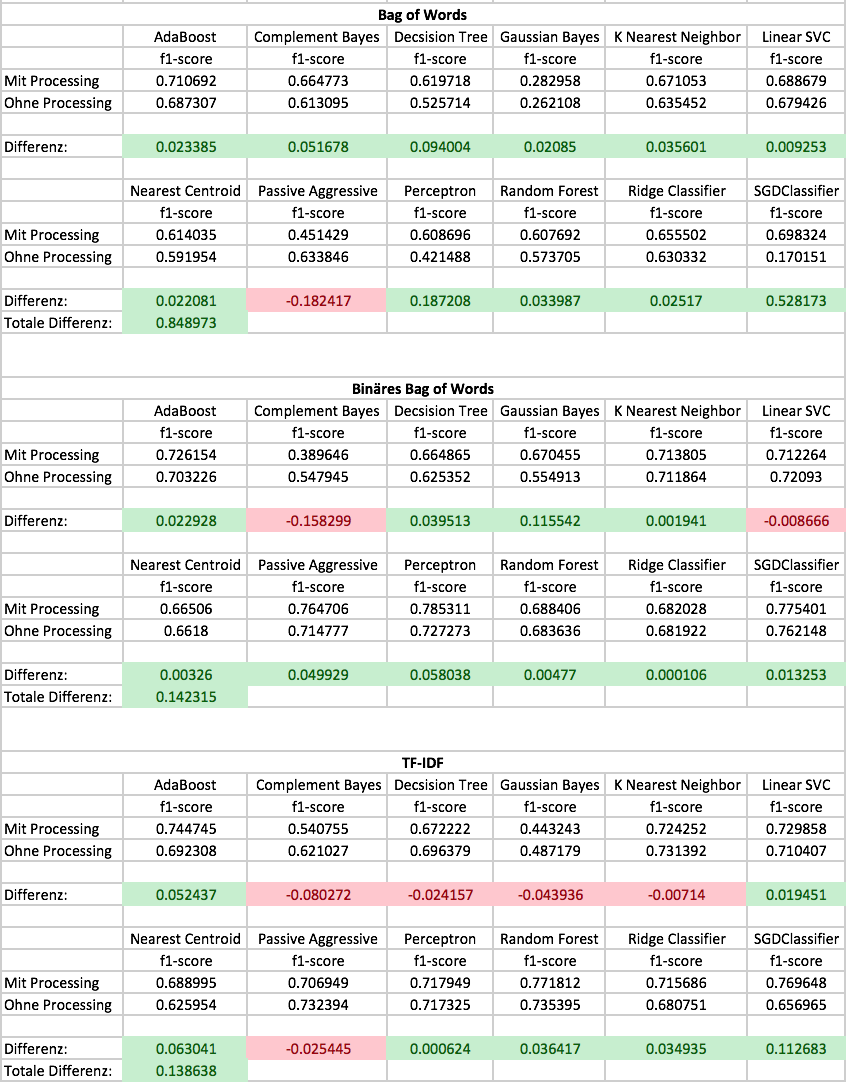
\includegraphics[width=1\columnwidth,keepaspectratio]{img/easypre.png}
	\caption{Grafik der Auswertung für einfaches Preprocessing}
\end{figure}
\subsubsection{Fortschrittliche Preprocessingschritte}
Das fortschrittliche Preprocessing erzielt bei allen drei Feature-Extraction Methoden keine eindeutigen Resultate.\\
Bei der \glqq Bag of Words\grqq{} Methode erreicht die Konfiguration \glqq config8\grqq{} mit dem Preisdetektor, der Stoppwörterentfernung und der Stammformreduktion die grössten positiven Einwirkungen.
Sieben Algorithmen können mit dieser Konfiguration ihre F1-Scores verbessern.
Somit wird für \glqq Bag of Words\grqq{} die Konfiguration \glqq config8\grqq{} weiter benutzt.\\
Bei der binären \glqq Bag of Words\grqq{} Methode gibt es bei keiner Konfiguration irgendwelche flächendeckenden Verbesserungen.
Es gibt jeweils nur vereinzelte Algorithmen, welche ihre Scores verbessern können.
Da keine Konfiguration eindeutig als Verbesserung angesehen werden kann, wird bei dieser Variante keine fortschrittlichen Preprocessingschritte angewendet.\\
Bei der TF-IDF-Methode gibt es ebenfalls keine eindeutigen Verbesserungen bei irgendeiner Konfiguration.
Es können vereinzelte Algorithmen ihre Scores verbessern, aber es findet nie flächendeckend eine Verbesserung statt.
Bei der Konfiguration \glqq config5\grqq{} erzielt AdaBoost den höchsten Wert über alle Konfigurationen gesehen, aber die anderen Algorithmen werden nur leicht beeinflusst.
Um bei der weiteren Ermittlung von Optimierungen nicht nur auf ein Algorithmus zu setzen, wird bei TF-IDF kein fortschrittliches Preprocessing angewendet.
\\\\
Die Auswertung für das fortschrittliche Preprocessing kann im Anhang gefunden werden.
\section{Klassifizieren mittels Machine-Learning}
\subsection{Dimensionsreduktion der Features}
Die Verwendung der Dimensionsreduktion mittels LSA erzielt bei allen drei Feature-Extraction Methoden deutliche Verbesserungen.
Der Grossteil der Algorithmen kann mit Hilfe von LSA den F1-Score verbessern.
Lediglich bei der \glqq Bag of Words\grqq{} Methode ist die Summe über alle Score-Verbesserungen negativ, dies jedoch nur, weil der Multinomial-Bayes Klassifizierer mit LSA einen stetigen F1-Score von null hat.\\
Die Dimensionsreduktion wird für alle drei Varianten weiter verwendet, da die positiven Auswirkungen sich deutlich in den F1-Scores widerspiegelt.
Einziger Wehrmutstropfen der Dimensionsreduktion ist, dass der Multinomial-Bayes Klassifizierer keine wirkliche Klassifizierung mehr durchführen kann.
Somit ist dieser Klassifizierer für den weiteren Verlauf nicht mehr verwendbar.
\begin{figure}[H]	
	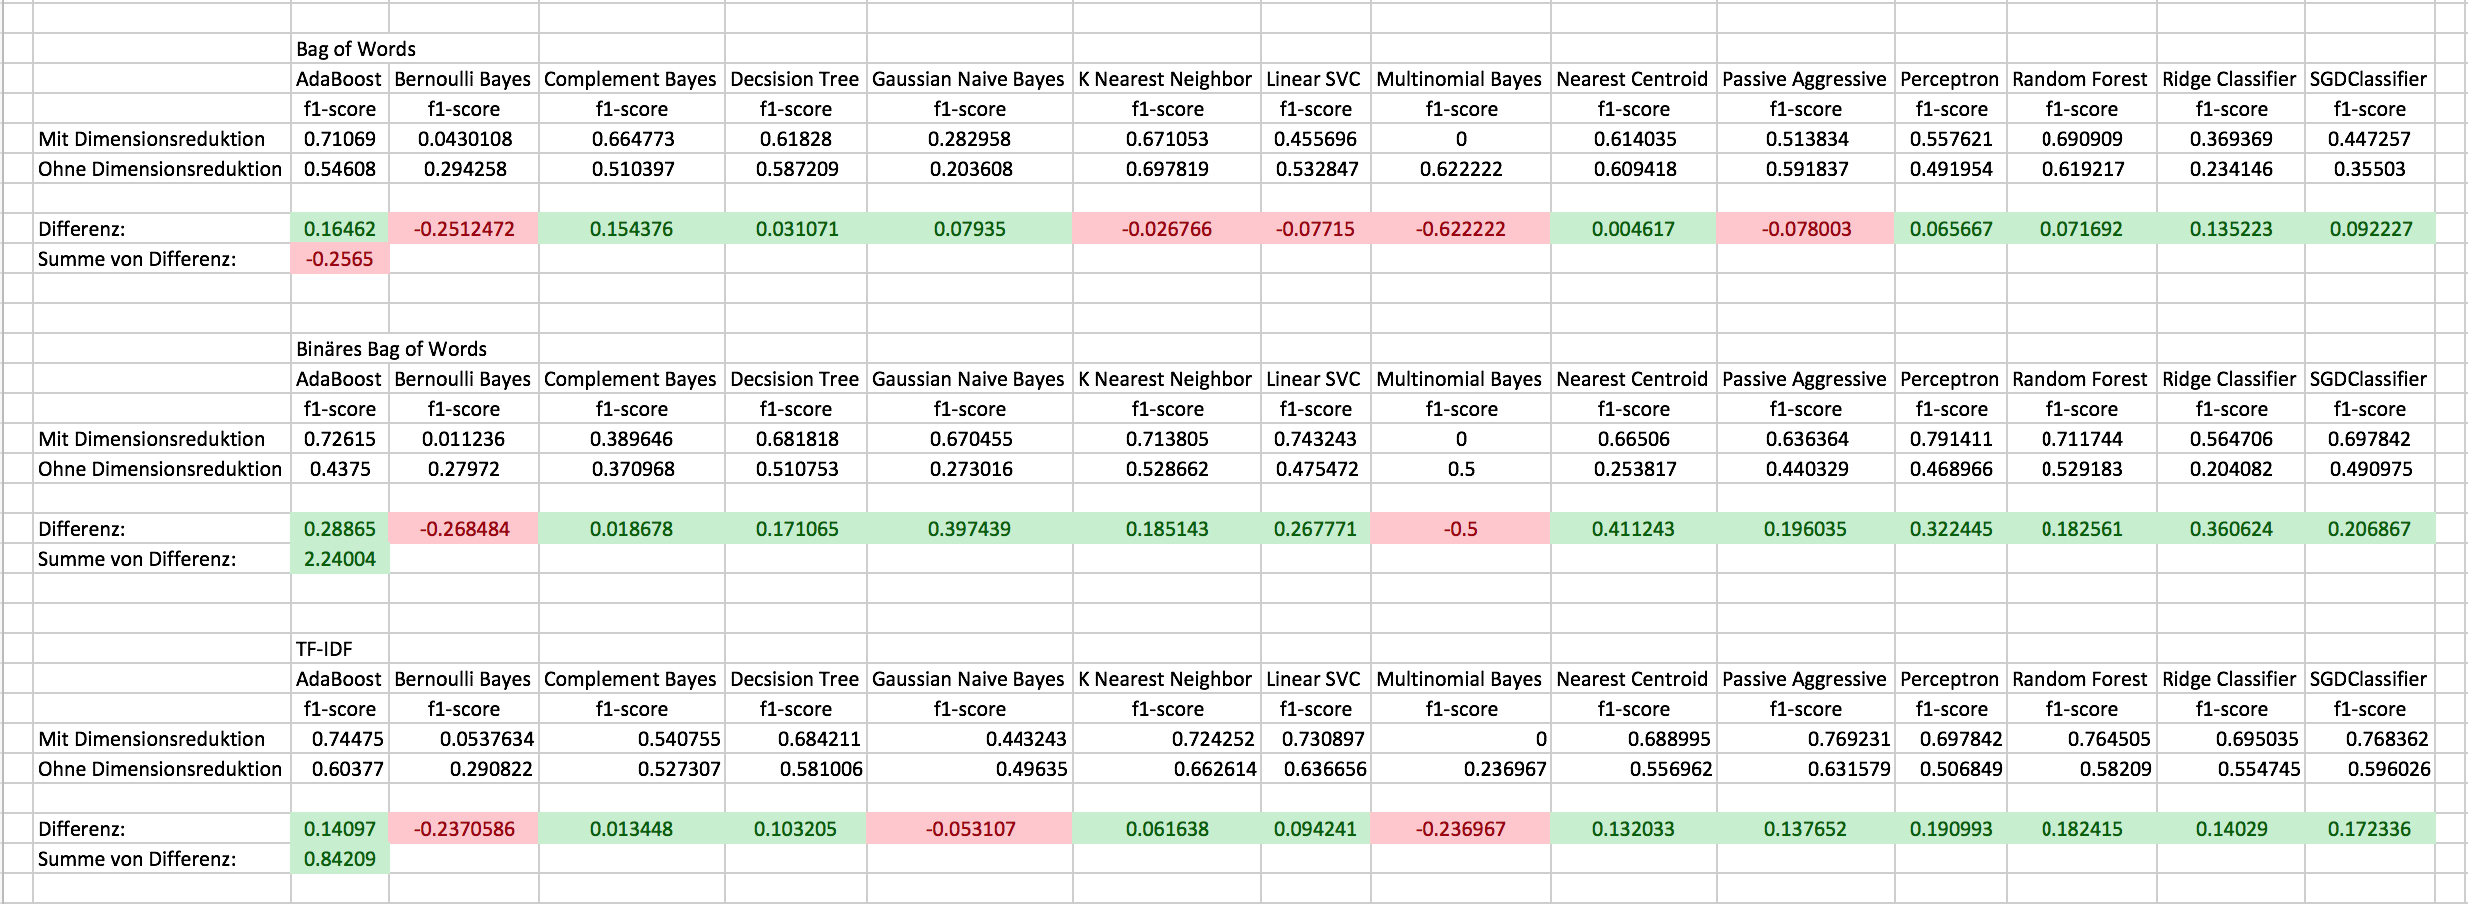
\includegraphics[width=1\columnwidth,keepaspectratio]{img/dimred.png}
	\caption{Grafik der Auswertung für die Dimensionsreduktion mittels LSA}
\end{figure}
\subsection{Klassenverteilung}
Die Angabe der Klassenverteilung konnte nicht bei allen Algorithmen als Parameter angegeben werden.
Somit werden alle Bayes-Algorithmen, KNearestNeighbor und Nearest-Centroid in dieser Auswertung nicht beachtet.\\
Bei beiden \glqq Bag of Words\grqq{} Methoden erzielt die Angabe der Klassenverteilung eine durchschnittliche Verbesserung der F1-Scores.
Einzelne Algorithmen reagieren negativ auf die Angabe, aber die positiven Auswirkungen übertreffen die negativen Auswirkungen.
Somit wird bei beiden \glqq Bag of Words\grqq{} Methoden die Angabe der Klassenverteilung miteinbezogen.\\
Bei der TF-IDF-Methode werden drei Algorithmen negativ und vier Algorithmen positiv beeinflusst.
Lediglich beim PassiveAgressiveClassifier gibt es eine markante Verschlechterung des F1-Scores.
Bei den anderen Algorithmen halten sich die negativen Auswirkungen im Rahmen.
Den F1-Score des PassiveAgressiveClassifier ausgenommen, sind die positiven Auswirkungen grösser als die negativen Auswirkungen.
Somit wird für TF-IDF ebenfalls die Angabe der Klassenverteilung für die nächsten Schritte beibehalten.
\begin{figure}[H]	
	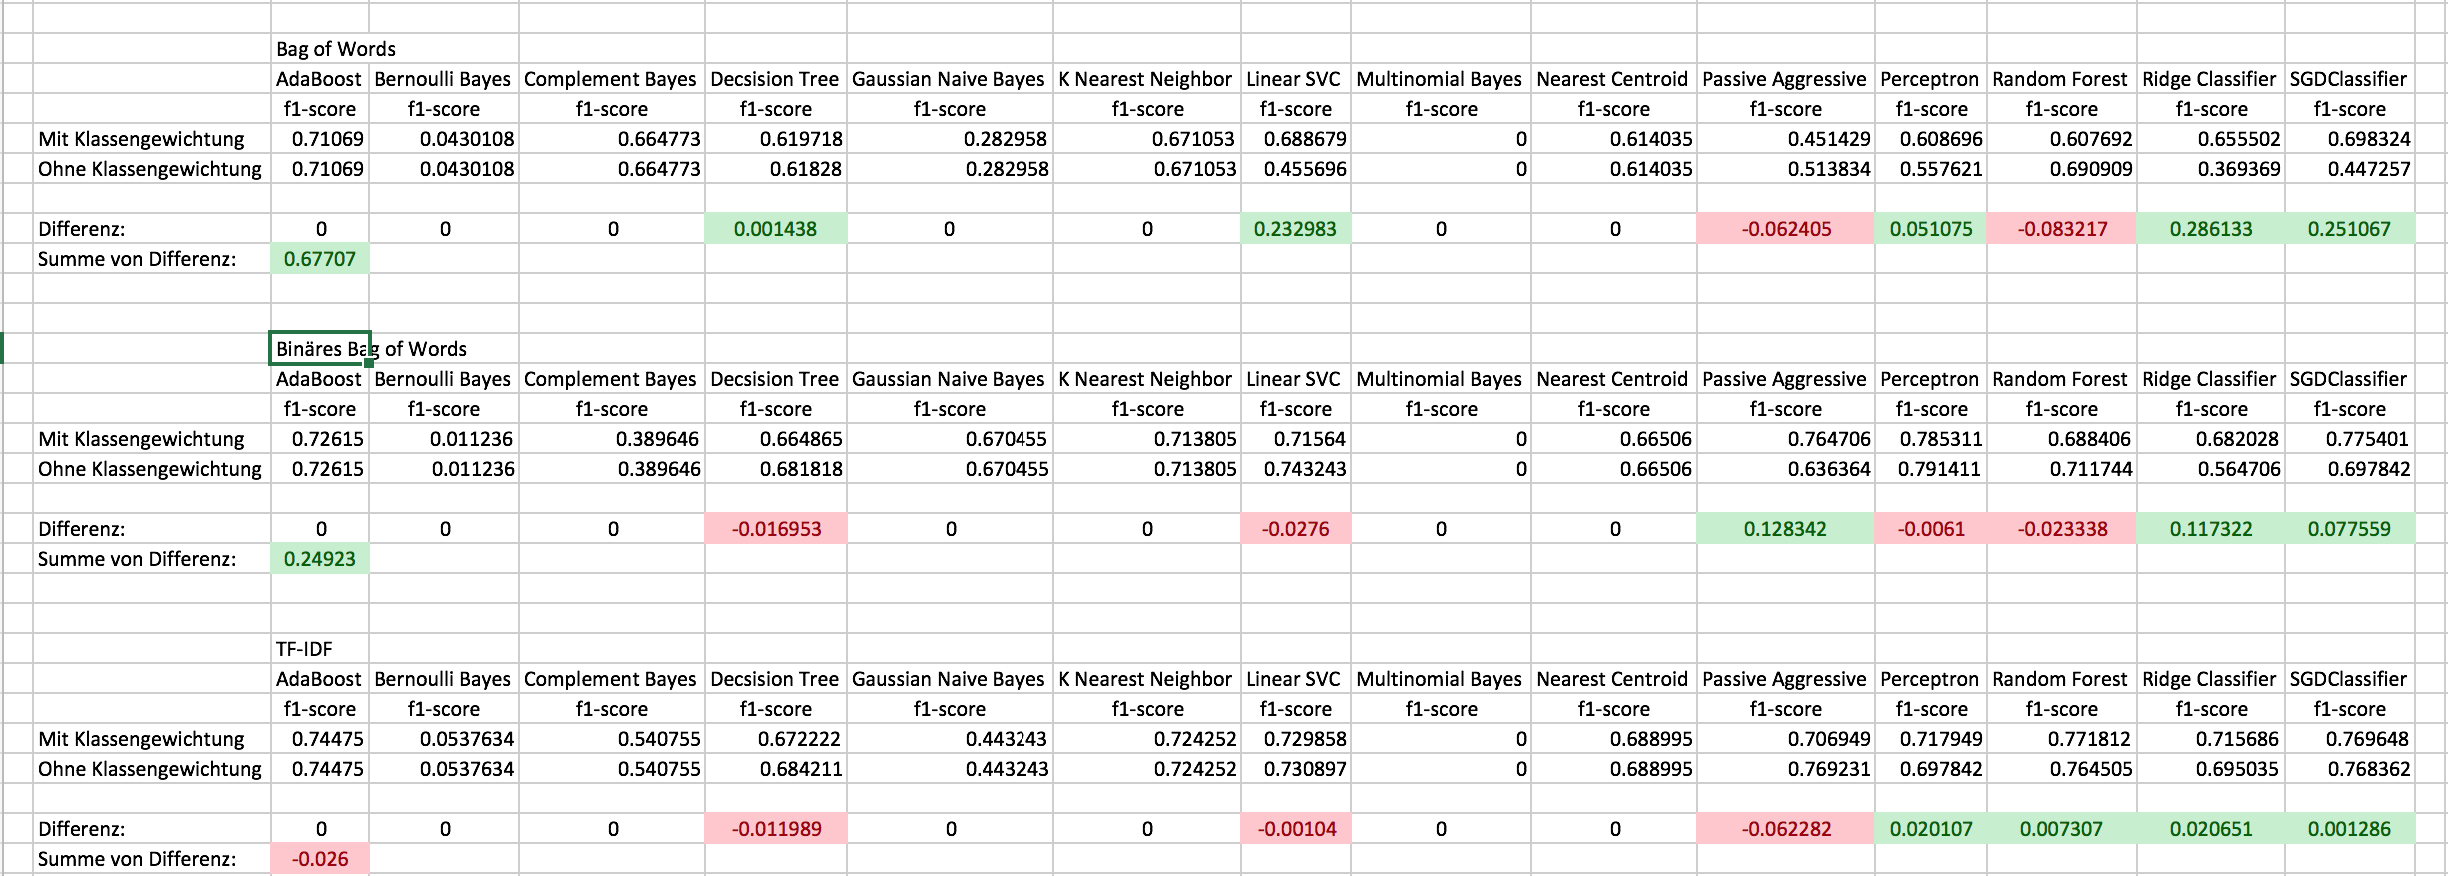
\includegraphics[width=1\columnwidth,keepaspectratio]{img/classweight.png}
	\caption{Grafik der Auswertung für die Klassenverteilung}
\end{figure}
\subsection{N-Gramme}
Sowohl \glqq Bag of Words\grqq{} als auch TF-IDF bieten in ihrer Scikit-Learn Implementierung die Möglichkeit N-Gramme zu verwenden.
Für dieses Experiment wurden Unigramme, Bigramme und Trigramme ausgetestet.\\
Bei beiden \glqq Bag of Words\grqq{} Methoden erzielt die Verwendung von Unigrammen die besten Ergebnisse.
Bi- und Trigramme können bei einzelnen Algorithmen ebenfalls eine Verbesserunge verzeichnen, aber im Vergleich zu Unigrammen fallen diese flächendeckend kleiner aus.
Somit werden bei beiden \glqq Bag of Words\grqq{} Varianten nur Unigramme verwendet.
Ebenfalls benötigt die Extrahierung der Features bei Bi- und Trigrammen circa doppelt so lange, was eine enorme Performanceeinbusse ist.\\
Bei der TF-IDF-Methode erzielen Bi- und Trigramme die exakt gleichen Werte.
Uni- und Bigramme erzielen im Durchschnitt ungefähr den gleichen Wert.
Bei der Verwendung von Unigrammen erzielt der Algorithmus Bernoulli-Bayes einen F1-Score von null.
Um nicht einen weiteren Algorithmus für die weiteren Schritte zu verlieren, wird deshalb die Verwendung von Bigrammen bei der TF-IDF-Methode verwendet.
\begin{figure}[H]	
	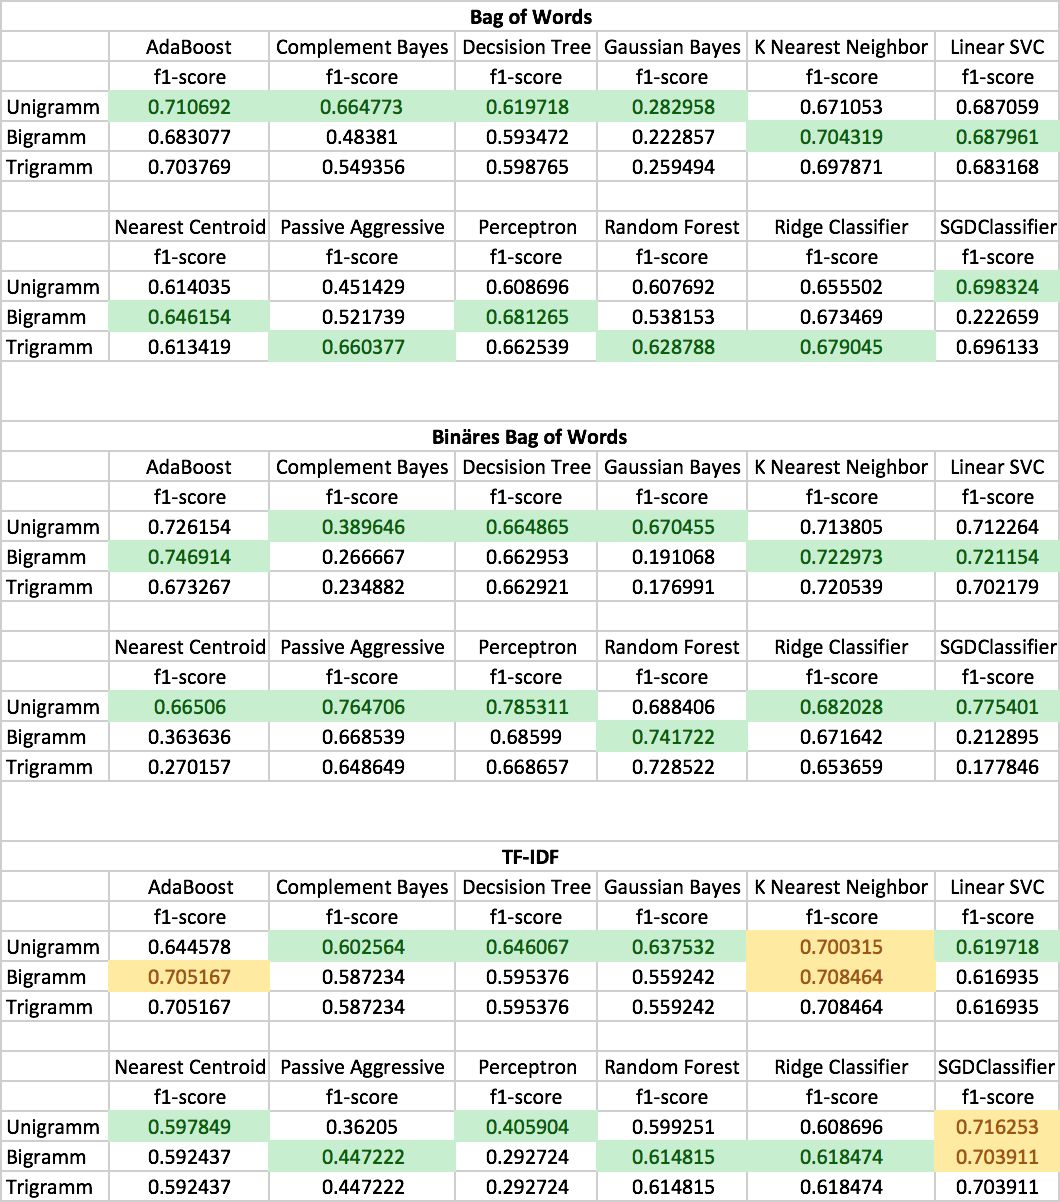
\includegraphics[width=1\columnwidth,keepaspectratio]{img/ngram.png}
	\caption{Grafik der N-Gramme Auswertung}
\end{figure}
\subsection{Anzahl extrahierter Features}
Für alle drei Feature-Extraction Methoden wurde ein Liniendiagramm für F1-Score, Precision und Recall erstellt.
Aus diesen Grafiken kann entnommen werden, bei welcher Feature-Anzahl welcher Algorithmus den besten Score erzielt.
Für die weitere Auswertung sind die Grafiken für F1-Score und Precision massgebend und werden weiter analysiert.
\subsubsection{Bag of Words}
Bei \glqq Bag of Words\grqq{} erzielt der Algorithmus AdaBoost bei 100 Features mit Abstand den besten F1-Score und erreicht fast die 0.8 Marke.
Ebenfalls kann der LinearSVC Algorithmus einen guten F1-Score erzielen und teilt sich mit AdaBoost die besten Werte.
Ersichtlich ist ebenfalls, dass die meisten Algorithmen sich zwischen 0.6 und 0.7 bewegen und das vereinzelte Klassifizierer mit ihren Werten auf und ab springen.\\
\begin{figure}[H]	
	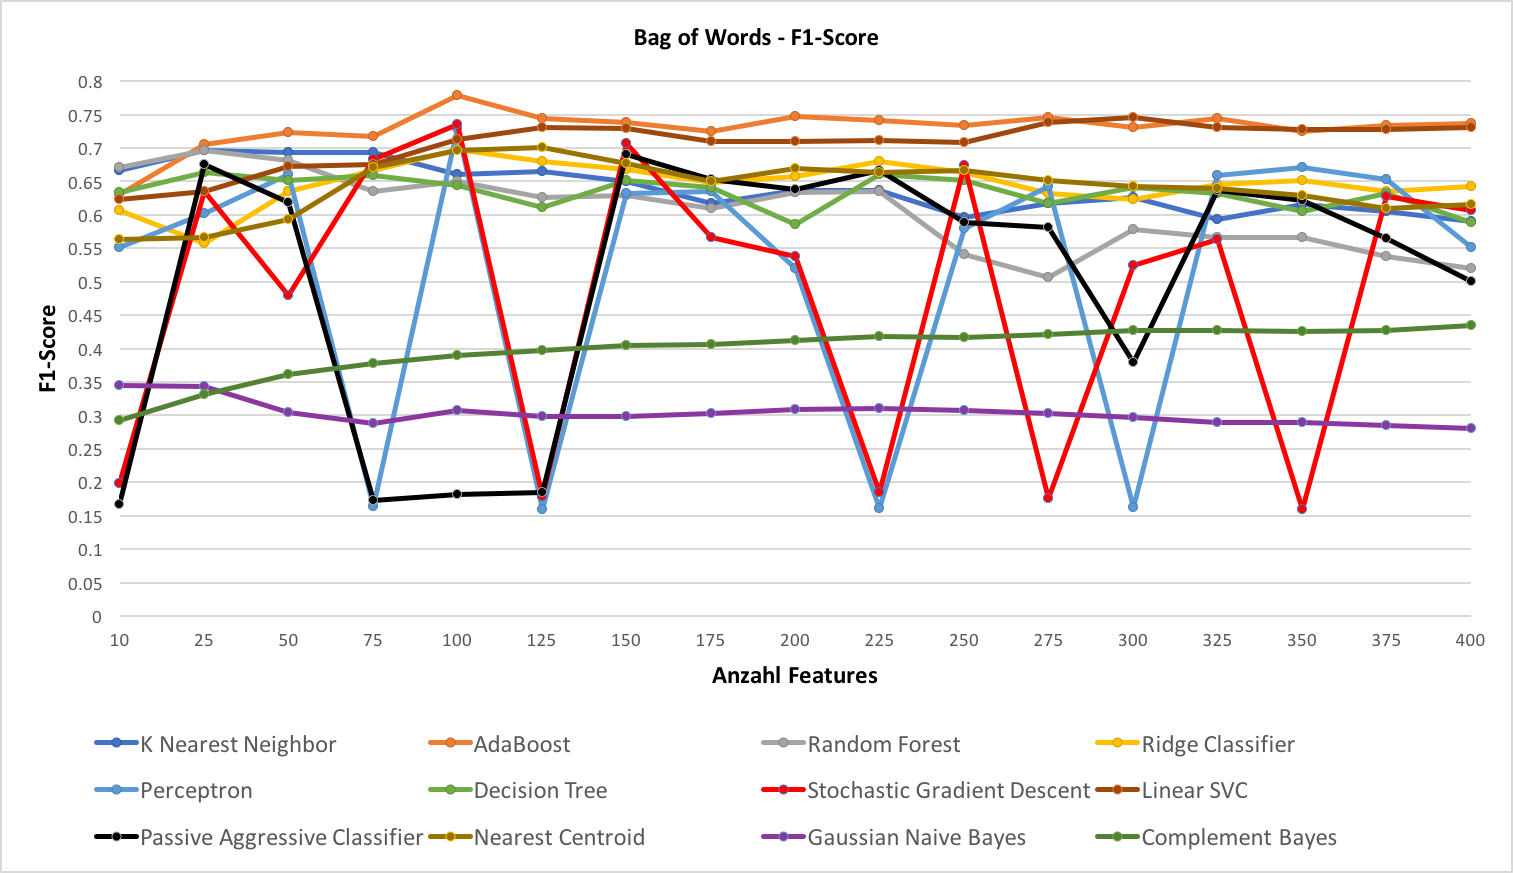
\includegraphics[width=0.8\columnwidth,keepaspectratio]{img/bow-f1.png}
	\caption{Grafik des F1-Score-Verlaufs bei Bag of Words}
\end{figure}
Bei der Precision ist der RandomForest Algorithmus der mit Abstand beste Klassifizierer.
Vereinzelt erreicht RandomForest eine Precision von 1.0 und ist stetig über 0.8.\\
Der Bernoulli-Bayes Algorithmus erreicht kurzzeitig ebenfalls eine Precision von eins, jedoch ist sein F1-Score jeweils unter 0.1.
Deswegen wir Bernoulli-Bayes nicht als ernsthafte Wahl angesehen und nicht beachtet.
\begin{figure}[H]	
	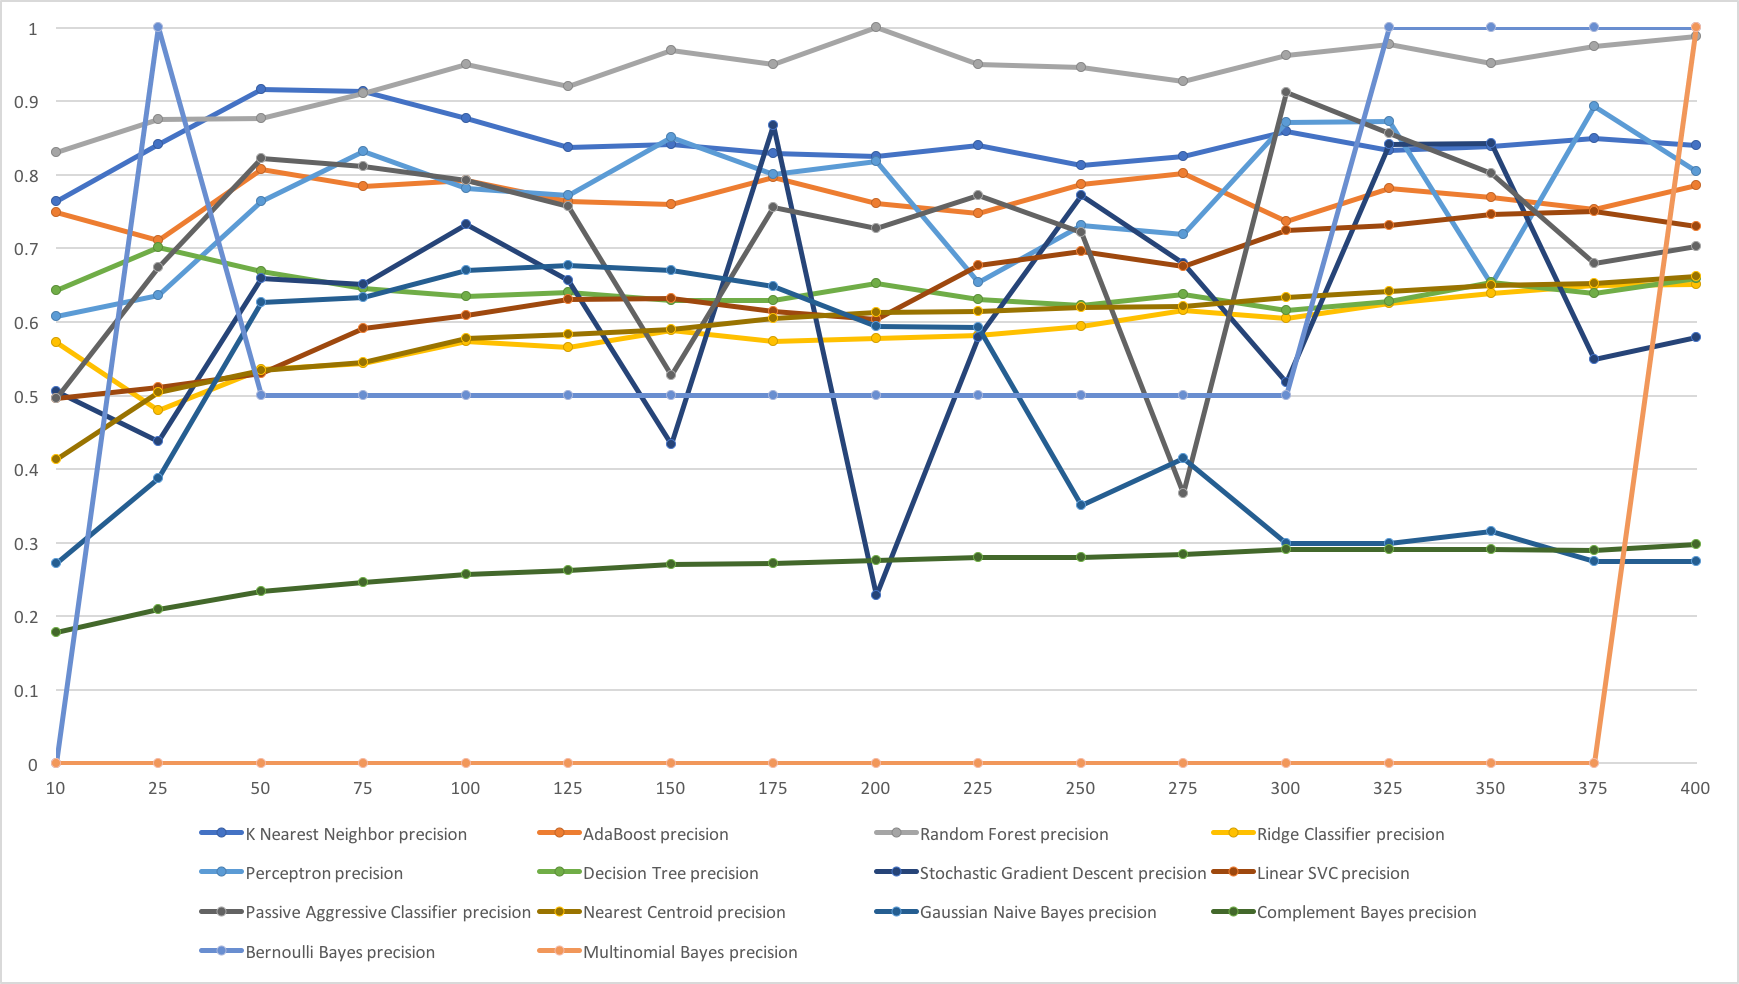
\includegraphics[width=0.8\columnwidth,keepaspectratio]{img/bow-pre.png}
	\caption{Grafik des Precision-Verlaufs bei Bag of Words}
\end{figure}
\subsubsection{Binäres Bag of Words}
Bei der Methode \glqq binäres Bag of Words\grqq{} können mehrere Algorithmen einen F1-Score nahe der 0.8 Grenze verbuchen.
Der beste Algorithmus ist Perceptron, welcher mit 325 Features einen F1-Score von 0.8 verzeichnet.\\
Der SGDClassifier erreicht ebenfalls einen F1-Score von 0.8, jedoch mit einer höheren Anzahl von Features.
Dies bedeutet das SGDClasifier potenziell länger für die Feature-Extraction benötigt und somit ist Perceptron der favorisierende Algorithmus bei dieser Variante.\\
\begin{figure}[H]	
	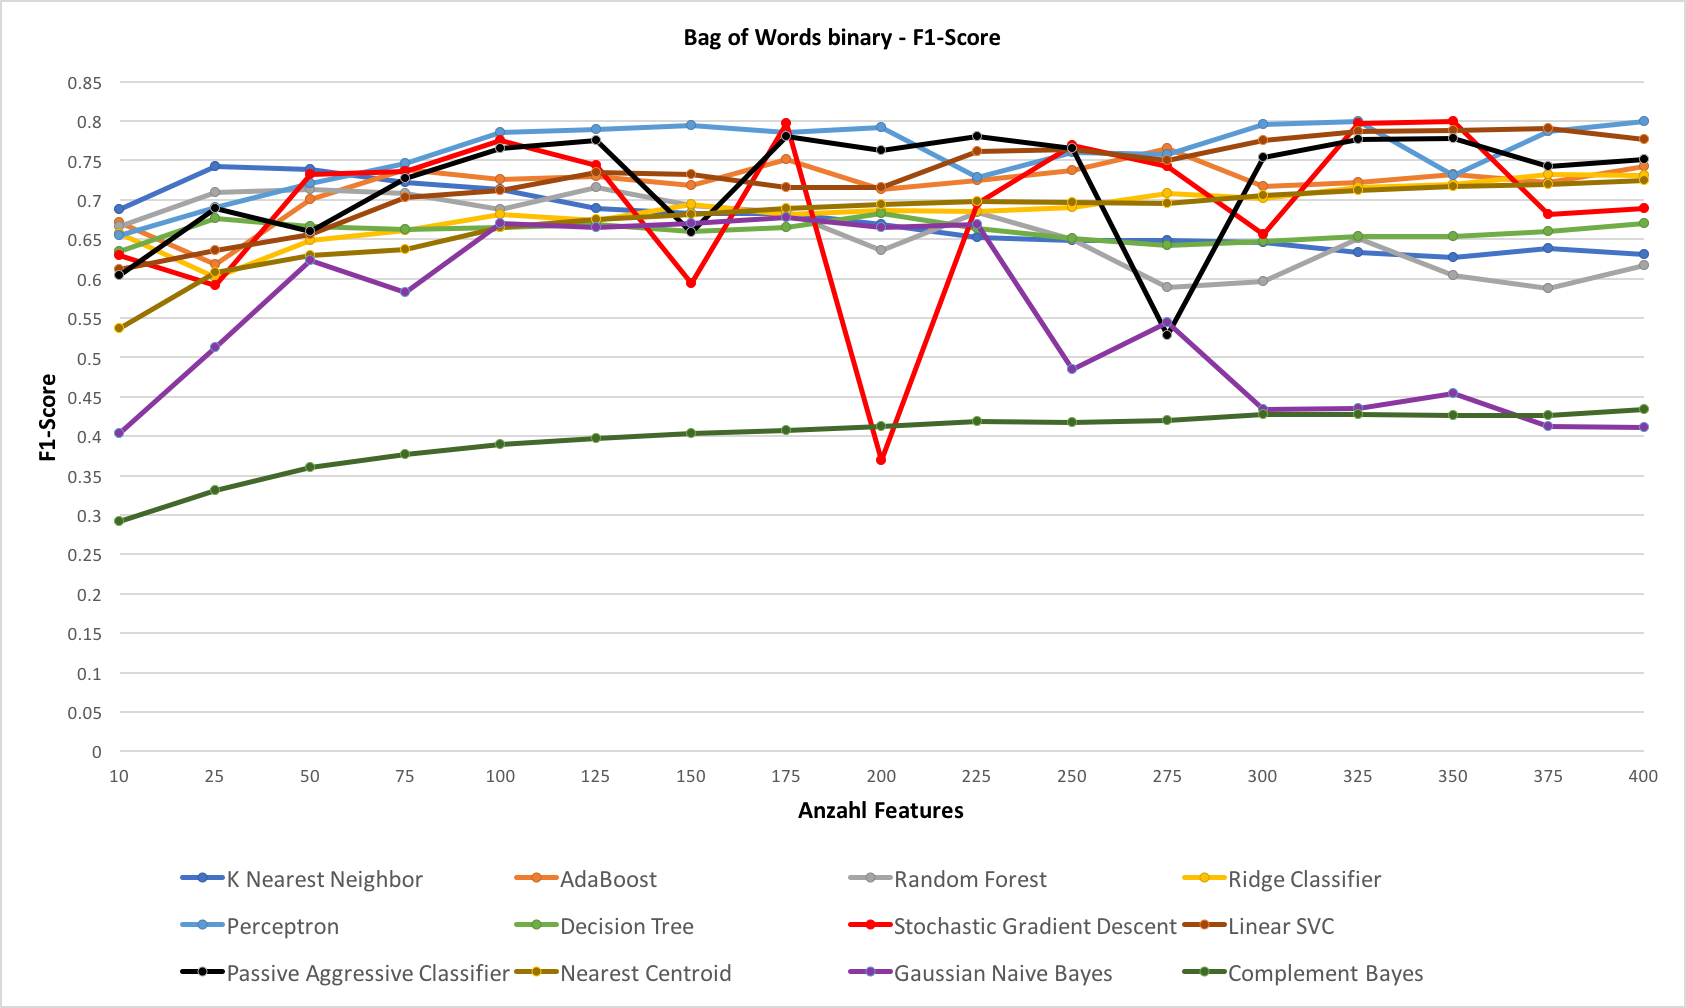
\includegraphics[width=0.8\columnwidth,keepaspectratio]{img/bow-bin-f1.png}
	\caption{Grafik des F1-Score-Verlaufs bei binärem Bag of Words}
\end{figure}
Bei der Precision ist der RandomForest Algorithmus ebenfalls die beste Wahl.
Er erreicht wieder die höchsten Prcecision-Werte bei einer vernünftigen Anzahl Features.\\
Ebenfalls springt der Bernoulli-Bayes wieder zwischen 1.0 und 0.5 umher.
Bei dieser Variante wird der Bernoulli-Bayes als keine Alternative gegenüber dem RandomForest in Betracht gezogen.
\begin{figure}[H]	
	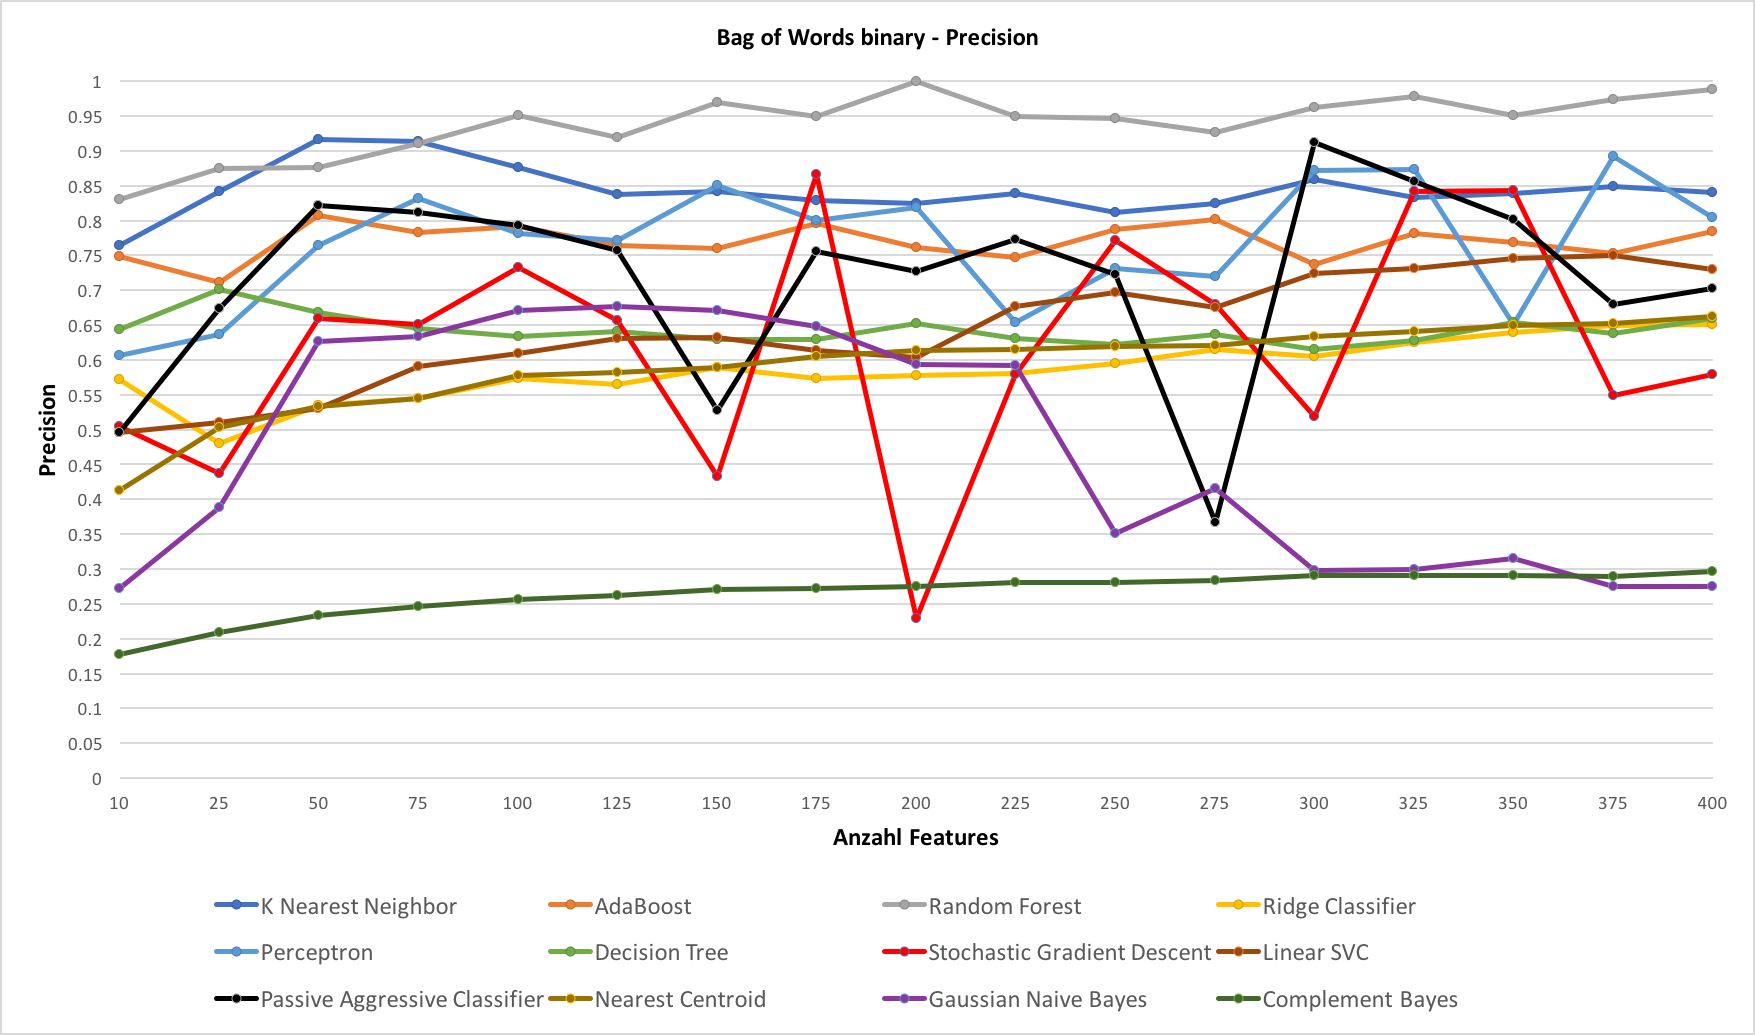
\includegraphics[width=0.8\columnwidth,keepaspectratio]{img/bow-bin-pre.png}
	\caption{Grafik des Precision-Verlaufs bei binärem Bag of Words}
\end{figure}
\subsubsection{TF-IDF}
Bei der Verwendung von TF-IDF sind mehrere Algorithmen mit ihren F1-Scores im Bereich 0.7 bis 0.8.
Der SGDClassifier Algorithmus kann als einziger die Grenze von 0.8 durchbrechen und ist somit der Algorithmus mit dem besten F1-Score.\\
\begin{figure}[H]	
	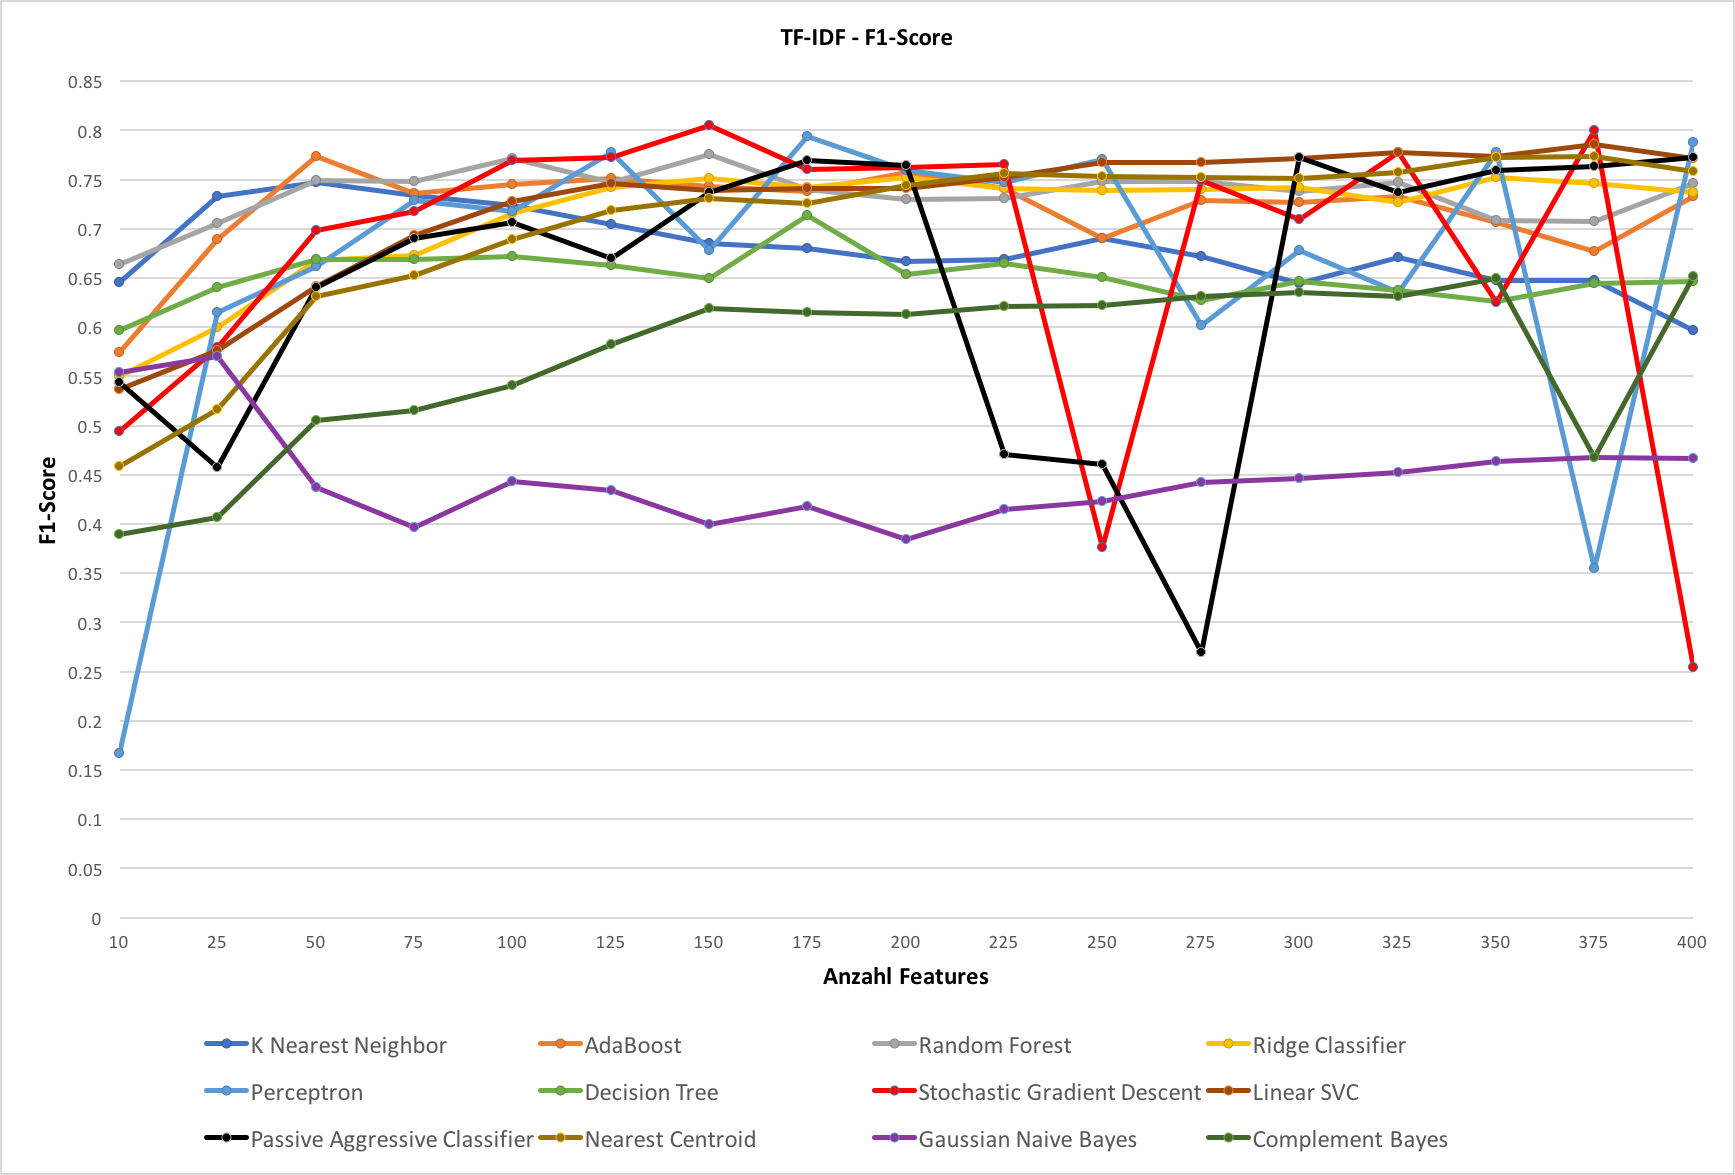
\includegraphics[width=0.8\columnwidth,keepaspectratio]{img/tfidf-f1.png}
	\caption{Grafik des F1-Score-Verlaufs bei TF-IDF}
\end{figure}
Bei der Precision ist der RandomForest Algorithmus ebenfalls wieder der Spitzenreiter.
Er erzielt bei fast jeder Anzahl von Features die beste Precision und kann bei 325 Features sein Maximum erreichen.
\begin{figure}[H]	
	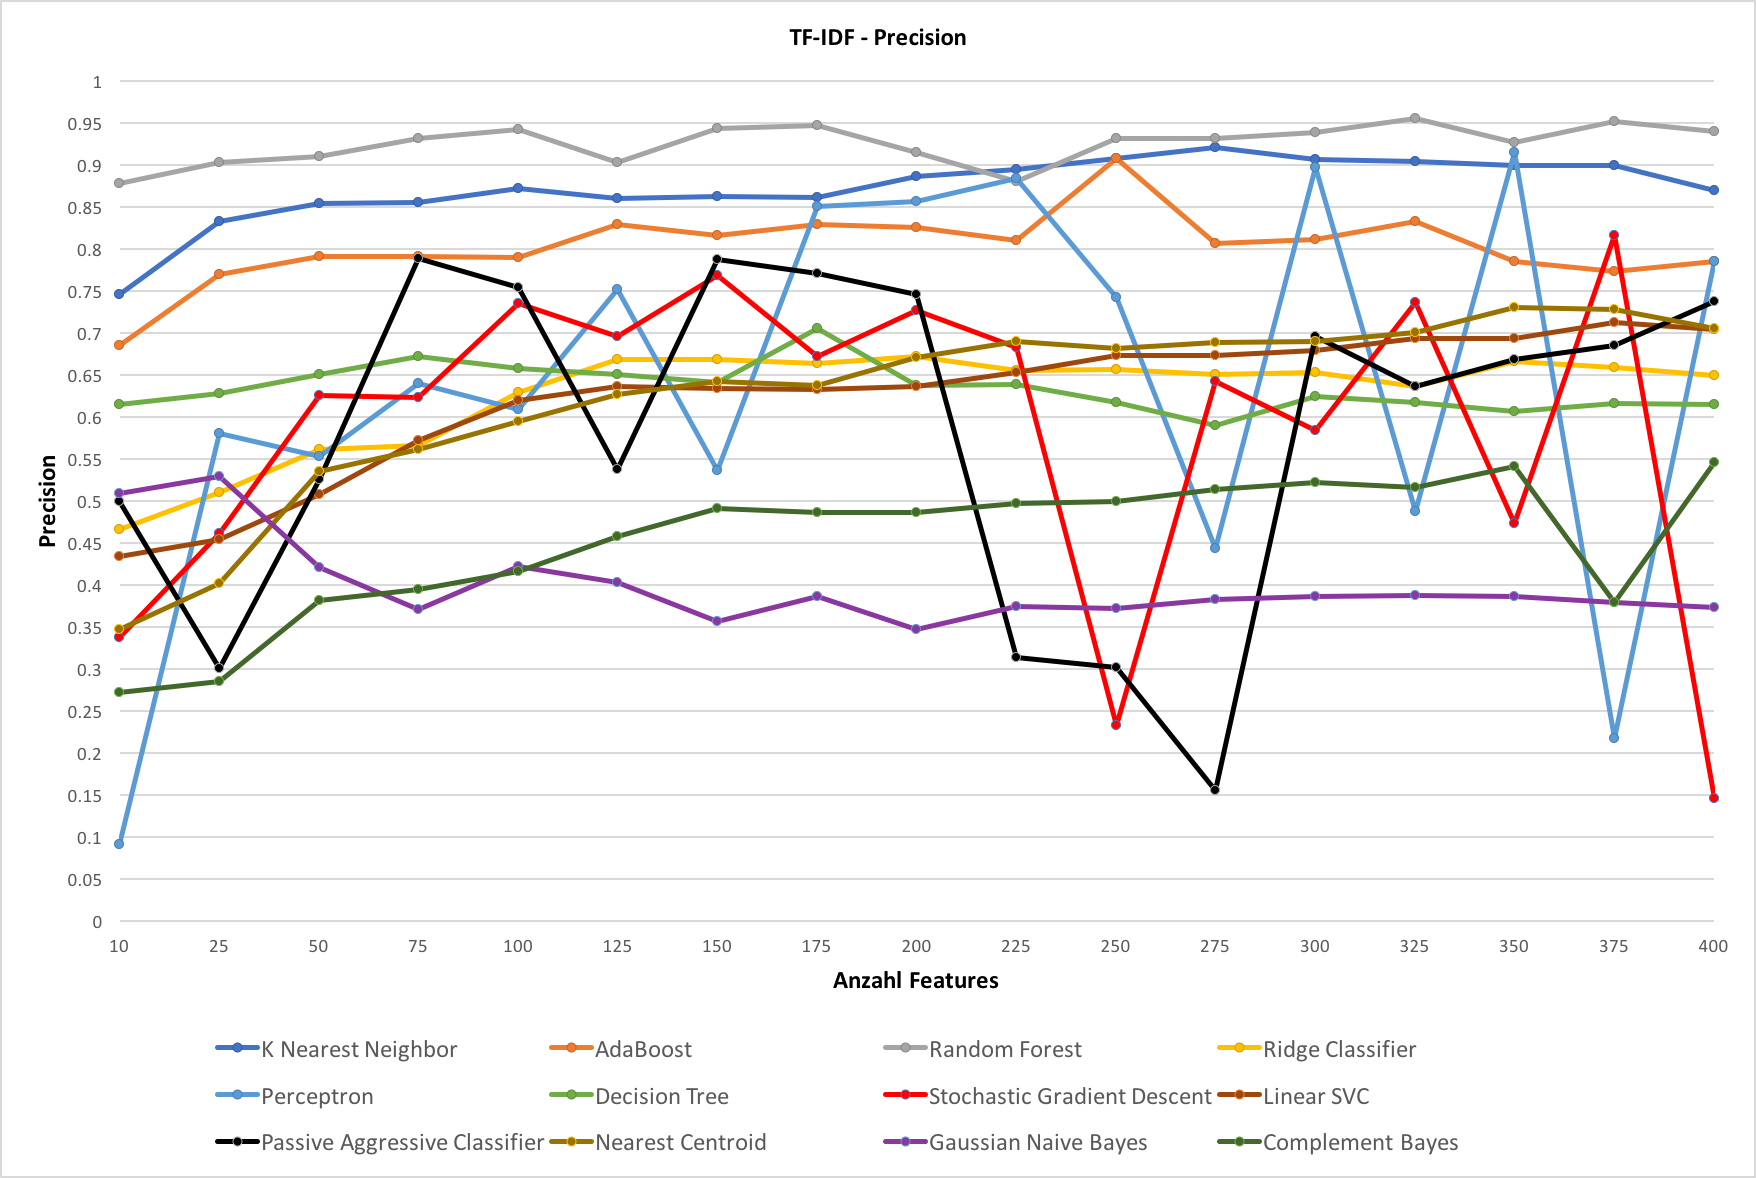
\includegraphics[width=0.8\columnwidth,keepaspectratio]{img/tfidf-pre.png}
	\caption{Grafik des Precision-Verlaufs bei TF-IDF}
\end{figure}
\subsection{Hyperparametertuning}
Die sechs Modelle, welche aus dem vorherigen Experiment, als die besten entnommen wurden, werden mittels Kreuzvalidierung auf optimale Hyperparameter durchsucht.
\subsubsection{Modelle mit bestem F1-Score}
Die drei Modelle AdaBoost, SGDClassifier und Perceptron können die besten F1-Scores erzielen.\\
\begin{table}[H]
	\caption{Auwertung Hyperparametertuning für AdaBoost mit binärem Bag of Words}
	\centering
	\begin{tabular}{|l|l|l|l|}
		\hline
		 & F1-Score & Precision & Recall\\
		\hline
		Vor Hyperparametertuning & 0.778 & 0.837 & 0.727 \\
		Nach Hyperparametertuning & 0.788 & 0.817 & 0.761 \\
		\hline
	\end{tabular}
\end{table}
\begin{table}[H]
	\caption{Auwertung Hyperparametertuning für Perceptron mit Bag of Words}
	\centering
	\begin{tabular}{|l|l|l|l|}
		\hline
		& F1-Score & Precision & Recall\\
		\hline
		Vor Hyperparametertuning & 0.8 & 0.872 & 0.739 \\
		Nach Hyperparametertuning & 0.579 & 0.426 & 0.903 \\
		\hline
	\end{tabular}
\end{table}
\begin{table}[H]
	\caption{Auwertung Hyperparametertuning für SGDClassifier mit TF-IDF}
	\centering
	\begin{tabular}{|l|l|l|l|}
		\hline
		& F1-Score & Precision & Recall\\
		\hline
		Vor Hyperparametertuning & 0.805 & 0.768 & 0.847 \\
		Nach Hyperparametertuning & 0.762 & 0.682 & 0.864 \\
		\hline
	\end{tabular}
\end{table}
Auffällig ist, dass AdaBoost als einziges Modell bessere Hyperparameter mittels Hyperparemtertuning finden konnte.\\
AdaBoost kann seinen Recall verbessern und gleichzeitig verschlechtert sich seine Precision.
Da die Recallsteigerung grösser als der Precisionabfall ist, wird der F1-Score nach oben korrigiert.\\
Die anderen beiden Modelle erzielen mit den neuen Parametern schlechtere Werte.
Beide können den Recall verbessern, jedoch müssen sie massive Gefälle bei der Precision einbüssen.
Da die Precision viel stärker abgenommen, als der Recall zugenommen hat, wird der F1-Score schlechter.\\
Perceptron hat im Vergleich zum SGDClassifier einen leicht tieferen F1-Score, jedoch ist seine Precision deutlich höher.
Da für den schlussendlichen \glqq Use-Case\grqq{} Precision wichtig ist, wird das Perceptron-Modell für weitere Auswertungen verwendet.
\subsubsection{Modelle mit bester Precision}
Das Modell RandomForest kann für alle drei Feature-Extraction Methoden jeweils den besten Precision-Score erzielen.\\
\begin{table}[H]
	\caption{Auwertung Hyperparametertuning für RandomForest mit binärem Bag of Words}
	\centering
	\begin{tabular}{|l|l|l|l|}
		\hline
		& F1-Score & Precision & Recall\\
		\hline
		Vor Hyperparametertuning & 0.636 & 1.0 & 0.466 \\
		Nach Hyperparametertuning & 0.736 & 0.8 & 0.682 \\
		\hline
	\end{tabular}
\end{table}
\begin{table}[H]
	\caption{Auwertung Hyperparametertuning für RandomForest mit Bag of Words}
	\centering
	\begin{tabular}{|l|l|l|l|}
		\hline
		& F1-Score & Precision & Recall\\
		\hline
		Vor Hyperparametertuning & 0.636 & 1.0 & 0.466 \\
		Nach Hyperparametertuning & 0.768 & 0.829 & 0.716 \\
		\hline
	\end{tabular}
\end{table}
\begin{table}[H]
	\caption{Auwertung Hyperparametertuning für RandomForest mit TF-IDF}
	\centering
	\begin{tabular}{|l|l|l|l|}
		\hline
		& F1-Score & Precision & Recall\\
		\hline
		Vor Hyperparametertuning & 0.747 & 0.956 & 0.614 \\
		Nach Hyperparametertuning & 0.794 & 0.823 & 0.767 \\
		\hline
	\end{tabular}
\end{table}
Alle drei Varianten können ihren F1-Score verbessern.
Die Verbesserung erfolgt nur im Bereich Recall, welcher initial bei allen drei Modellen relativ tief war.
Zusätzlich sinken bei allen drei Modellen die Precision-Scores.
Bei beiden Varianten mit Bag of Words, waren alle drei initialen Scores identisch und die Precision maximal.\\
Da in diesem Abschnitt auf die beste Precision geachtet wird, ist das Modell mit binärem Bag of Words und mit den Standardparametern die beste Variante.
